##
Just checking





<the sprint stuff should really go here...>









\begin{figure}[H]
\centering
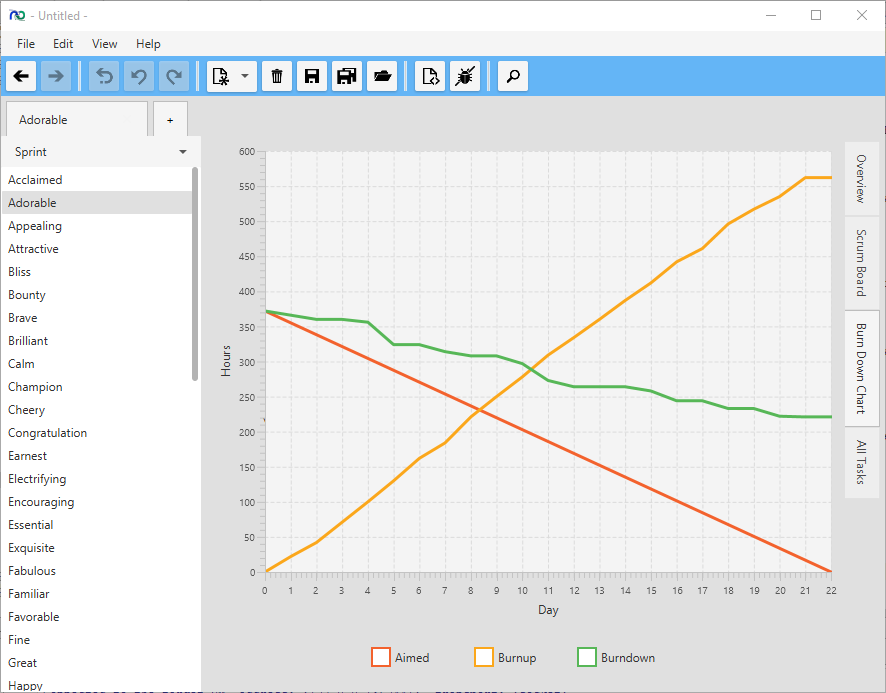
\includegraphics[width=\textwidth]{images/screenshots/burndown.png}
\caption{An example burndown chart}
\label{fig:burndown}
\end{figure}

Switching to the burndown tab will show a burndown graph for the currently selected sprint.

\textbf{Note:}\newline
A graph will only be shown if the sprint is past its start date and it has tasks. In these circumstances an error message will be shown instead.